\documentclass{../res/univ-projet}
\usepackage{graphicx}
\usepackage[francais]{babel}
\usepackage[T1]{fontenc}
\usepackage[utf8]{inputenc}
\usepackage{algorithmic}
\usepackage{algorithm}
\usepackage{dsfont}



\title{\'Etude du système d'OTP \og{}HOTP\fg{}}
\author{Les chats sauvages}

\projet{One Time Project}
\projdesc{\'Etude des syst\`emes de mots de passe jetable}
\filiere{M1SSI}
\logo{../res/logo_univ.png}


\graphicspath{{imgHOTP/}}


\begin{document}
\maketitle

\begin{abstract}
Ce document présente une analyse du système d'OTP \og{}HOTP\fg{}. Toutes les informations présentées et analysées proviennent des RFCs 4226 et 2104 ainsi que 
de leurs correctifs. Le but de cet article est de déterminer dans quelle mesure le système HOTP est utilisable, sous quelles conditions et avec quelles garanties de 
sécurité.Ce documents sera mis en relation avec plusieurs autres afin de réaliser un comparatif entre les systèmes d'OTP majeurs.
\end{abstract}
\newpage
\tableofcontents
\newpage

\section{Pré-requis}
Le système d'OTP \og{}HOTP\fg{} est un système d'authentification par mot de passe jetable qui étend le système le système OTP définit dans la RFC 2289. Le système OTP 
est étudié plus haut.
Le système HOTP repose principalement sur l'utilisation du mécanisme d'authentification de message HMAC. Ce mécanisme destiné à vérifier si un message n'a pas été altéré
et à authentifier l'expéditeur, repose lui-même sur l'utilisation d'une fonction de hachage et d'un secret partagé. La ou un mécanisme classique de vérification 
d'intégrité de message se contente de hacher ce dernier pour obtenir une empreinte, le mécanisme HMAC utilise une clef secrète pour authentifier l'expéditeur. Cette clef 
est prise en compte de la manière suivante : 
\begin{center}
$HMAC_K(M) = h(K \oplus opad || h(K \oplus ipad || M))$ 
\end{center}
où :\newline
$K$ est la clef secrète \newline
$opad$ = 0x36 répété un certain nombre de fois \newline
$ipad$ = 0x5C répété le m\^eme nombre de fois \newline
$\oplus$ est l'opération XOR \newline
$M$ est le message \newline


Dans le cadre de l'authentification de messages, le code HMAC du texte sera envoyé au destinataire sur un canal sécurisé différent de celui utilisé pour la transmission
du message. Le destinataire, une fois le message et le code HMAC reçus, pourra vérifier l'authenticité du message en calculant le code HMAC de ce dernier et en le 
comparant avec celui envoyé.

Le mécanisme HMAC sera ici utilisé pour la génération de mots de passes jetables.

\section{Généralités}
Lors de l'utilisation d'un système de mot de passe jetable le client (ou plus généralement l'entité souhaitant s'authentifier sur le service) fournit au service un 
classique login et un mot de passe. Contrairement aux méthodes classiques d'authentification par login et mot de passe, ici le mot de passe n'est utilisable qu'une seule et 
unique fois et sera donc différent à chaque connexion.
Il existe deux grandes catégories de système de mots de passe jetable : les systèmes dits \og{}synchrones\fg{} et les systèmes dits \og{}asynchrones\fg{}. Les premiers 
reposent sur le partage d'un secret entre le client et le serveur ainsi que sur un élément de synchronisation (i.e un compteur partagé, l'heure actuelle...). Les seconds 
au contraire ne reposent que sur le partage du secret et ne demandent aucune synchronisation entre client et serveur.
Le système \og{}HOTP\fg{} étudié ici est synchrone. Sont principe de fonctionnement est le suivant :
\begin{itemize}
 \item L'utilisateur demande à son token\footnote{Le token est un élément matériel ou logiciel dont la seule fonction est de générer des mots de passe jetables.} de 
 générer un mot de passe jetable.
 \item Le token génère le mot de passe en calculant $HMAC_K(C)$, avec K le secret partagé et C le compteur de synchronisation, puis incrémente le compteur.
 \item L'utilisateur récupère le mot de passe jetable fourni par le token et le passe au serveur d'authentification.
 \item Le serveur calcule la valeur de $HMAC_K(C)$, avec K le secret partagé et le compteur de synchronisation, puis incrémente le compteur.
 \item Si la valeur calculée par le serveur coïncide avec la valeur envoyée par l'utilisateur, ce dernier est authentifié. Dans le cas contraire, il est rejeté
\end{itemize}

Le principal intérêt des méthodes d'authentification par mot de passe jetable, et donc de la méthode HOTP, est d'éviter les attaques dites \og{}par rejeu\fg{} durant 
lesquelles un attaquant récupère le mot de passe durant une communication client-serveur et l'utilise ensuite pour usurper l'identité du client.

\section{Approfondissement}
  Étudions maintenant le fonctionnement précis du système de mot de passe jetable \og{}HOTP\fg{}.
  \subsection{Génération et partage d'un secret}
    Le secret partagé entre le client et le serveur est le point le plus sensible du système d'authentification par mot de passe jetable. En effet, si un attaquant 
    parvient à s'emparer du secret d'un utilisateur, il sera capable de s'authentifier à sa place, mettant en péril la sécurité du compte utilisateur. La méthode 
    \og{}HOTP\fg{} propose pour la génération des secrets deux méthodes : une méthode déterministe et une méthode aléatoire. Détaillons ces deux méthodes.
    
    \subsubsection{Méthode déterministe}
    Pour la méthode déterministe, une clef maitresse, notée $K_M$ doit être enregistrée sur le serveur. Puisque les clefs secrètes de tous les clients seront dérivées 
    de $K_M$, cette clef devra être stockée dans une zone très sécurisée voir inviolable. Lorsque qu'un nouveau client sera ajouté au service de connexion, celui ci
    se verra muni d'une clef secrète, $K_i$, personnelle qui sera partagée avec le serveur. Cette clef sera calculée à partir de la clef $K_M$ et d'une information, $i$, 
    identifiant le client de la manière suivante : \newline
    \begin{center}
     $K_i = h(K_M || i)$ 
    \end{center}
    \hfill{},avec h une fonction de hachage.\newline
    Cette clef constitue un secret unique et robuste si l'on respecte les conditions suivante :
    \begin{itemize}
     \item La fonction $h$ est une fonction de hachage non inversible (md5, SHA\_1...).
     \item Le secret $K_M$ est inviolable.
     \item Le paramètre $i$ est un identifiant unique à chaque utilisateur (ID matériel, numéro de série...)
    \end{itemize}
    
    \subsubsection{Méthode aléatoire}
    Pour la seconde méthode, une clef aléatoire est générée pour chaque nouveau client demandant l'association.
    Afin d'assurer la robustesse du secret, le générateur aléatoire doit être choisi le moins prédictible possible. Il est en général préférable de choisir un générateur 
    matériel, reposant sur l'aléatoire d'un phénomène physique (décomposition de noyaux atomiques, bruit thermique...). A défaut, un très bon générateur pseudo-aléatoire 
    reposant sur l'exécution d'un algorithme (\emph{Yarrow}, \emph{Fortuna}, \emph{Blum Blum Shub}, \emph{ISAAC}...) peut être utilisé. Quel que soit le générateur 
    utilisé, celui ci doit fournir une sortie imprédictible et une distribution de probabilité entre les clefs aussi uniforme que possible.
  
  Quelle que soit la méthode de génération utilisée, la clef produite doit être d'une longueur correspondant aux standards de sécurité actuels. A l'heure ou ce rapport 
  est écrit, une longueur de clef de 128 bits parait être un minimum. Choisir une longueur supérieure ou égale à 160 bits semble plus raisonnable et une clef de 256 
  bits ou plus fournit un très bon niveau de sécurité.
    
  \subsection{Génération d'un mot de passe jetable}
  La génération d'un OTP avec la méthode HOTP repose sur l'utilisation d'un compteur incrémental et de la clef secrète, tous deux partagés entre le token et le service de 
  validation. Une fonction HMAC définie pour une fonction de hachage donnée est aussi utilisée pour produire la base de l'OTP.
  Au global, la génération de l'OTP se décompose en trois étapes principales selon l'algorithme \ref{HOTP:gene}.
  \begin{algorithm}
  \caption{Génération d'un OTP par HOTP}
    \label{HOTP:gene}
   
    \begin{algorithmic}
    \REQUIRE $K$ une clef secrète, $C$ un compteur de synchronisation.
    \STATE $HVal \leftarrow HMAC(K, C)$
    \STATE $HVal \leftarrow tronc(HVal)$
    \STATE $HVal \leftarrow binToDec(HVal)$
    \STATE $C \leftarrow C + 1$
    \newline
    \RETURN $HVal \bmod 10^L$ // L : longueur souhaitée de l'OTP
    \end{algorithmic}
  \end{algorithm}
  
  Dans ce schéma, la première étape consiste à calculer la valeur de HMAC pour la clé secrète partagée et en prenant pour message le compteur de synchronisation. La 
  longueur de la valeur obtenue dépend de la fonction de hachage utilisée. On aura par exemple une chaine de 160 bits en utilisant la fonction SHA\_1.
  On pourrait utiliser la sortie de la fonction HMAC comme OTP cependant, écrite en décimal cette valeur se représenterait sur 48 chiffres et serait peut pratique à entrer 
  pour un utilisateur. C'est pourquoi les étapes 2 et 3 vont permettre de réduire la longueur de l'OTP à une valeur sur 10 chiffres via les fonctions $tronc$ et 
  $binToDec$. La fonction $tronc$, qui extrait une chaine de 31 bits de la sortie de $HMAC$, est définie par l'algorithme \ref{HOTP:trunc}.
  
  \begin{algorithm}
    \caption{tronc : Réduction de la sortie de $HMAC$}
    \label{HOTP:trunc}
    
    \begin{algorithmic}
      \REQUIRE S une chaine de bit
      \ENSURE S est de longueur 31 bits
      \STATE $offBits \leftarrow$ Les 4 bits de poids faible de S[19]
      \STATE $offset \leftarrow binToDec(offBits)$ // 0 $\leq offset \leq$ 15
      \STATE $P \leftarrow S[offset]..S[offset + 3]$ \newline
      \RETURN Les 31 derniers bits de $P$
    \end{algorithmic}
  \end{algorithm}

  La fonction $binToDec$, quant à elle, va convertir la chaine binaire retournée par $tronc$ en un nombre décimal, composé de 10 chiffres. Afin de faciliter encore un peu 
  plus la saisie du mot de passe jetable, on ne conservera qu'une partie du nombre à 10 chiffres en en prenant le modulo $10^P$, o\`u P est la longueur souhaitée de l'OTP.
  Afin que le mot de passe soit à la fois facilement utilisable et sécurisé, il est conseillé de choisir une valeur de $P$ comprise entre 6 et 8 inclus.
  Après la génération du mot de passe, le compteur de synchronisation est incrémenté pour garantir l'unicité de la valeur produite.
  
  \subsection{Soumission et protocole de vérification}
  La soumission du mot de passe jetable est, pour HOTP, indépendante du reste du système. Dans la majorité des cas, cette étape passera par l'utilisation d'une interface 
  de connexion graphique ou en ligne de commande. Nous nous intéresserons dans cette section à la partie vérification du mot de passe par le serveur. Cette étape est 
  décrite dans l'algorithme \ref{HOTP:verif}.  
  \begin{algorithm}
    \caption{Vérification d'un mot de passe jetable.}
    \label{HOTP:verif}
    
    \begin{algorithmic}
      \STATE $attentNB \leftarrow 0$
      \STATE $C \leftarrow$ compteur de synchronisation de l'utilisateur
      \STATE $K \leftarrow$ clef secrète de l'utilisateur
      \STATE $OTP_1 \leftarrow HOTP_K(C)$
      \WHILE{$attentNB < MAX\_ATTENT$}
	\STATE $OTP_2 \leftarrow$ récupérer\_OTP
	\STATE $attentNB \leftarrow attentNB + 1$
	\IF{$OTP_1 = OTP_2$}
	  \STATE $C \leftarrow C + 1$
	  \STATE accepter l'utilisateur
	\ELSE
	  \IF{resynchro possible}
	    \STATE $resynchro$
	    \STATE accepter l'utilisateur
	  \ENDIF
	\ENDIF
      \ENDWHILE
      \STATE $verouiller$
      \STATE $prevenir$
    \end{algorithmic}
  \end{algorithm}
  
  Dans cet algorithme, la variable $attentNB$ représente le nombre de tentatives d'OTP déjà effectuées par l'utilisateur. Elle permet de contrôler le nombre maximal de mots 
  de passes entrés entre deux authentification réussies dans le but d'éviter les attaque par \emph{brute force}.
  L'algorithme nécessite aussi de connaitre la clef secrète et le compteur de synchronisation liés à l'utilisateur. Le mode de récupération de ces informations n'est pas 
  détaillé dans cet algorithme puisqu'il est complètement indépendant de la méthode HOTP. Dans la majorité des cas, ces informations seront stockées dans une base de 
  données et la récupération se résumera donc à une requête sur cette dernière. Il n'est pas possible de se passer de ces deux informations puisque le serveur 
  d'authentification doit être capable de calculer la valeur de $HOTP_K(C)$ de la même manière que le token de l'utilisateur afin de vérifier l'exactitude la valeur 
  reçue.
  
  Dans sa généralité, l'algorithme de vérification ressemble fortement à un algorithme d'authentification par login / mot de passe standard. A savoir, on demande à 
  l'utilisateur de fournir ses paramètres de connexion et on les vérifie. Si les données passées s'avèrent correctes, l'utilisateur est authentifié, sinon on recommence 
  l'opération jusqu'à l'obtention de données correctes ou jusqu'à atteindre le nombre maximal de tentative. Cependant, on retrouve une différence dans l'appel aux 
  fonctions \og{}resynchro possible\fg{} et \og{}resynchro\fg{}. Ces fonctions, détaillées dans la section \ref{HOTP:synchro}, on pour but d'assurer la cohérence du 
  compteur de synchronisation partagé.
  
  \subsection{Synchronisation}
  \label{HOTP:synchro}
  Par nature, le système HOTP requière que les compteurs du serveur et du token soient synchronisés. En effet, dans le cas contraire, les valeurs de l'OTP calculées par le 
  token et le service d'authentification seraient différentes et aucun utilisateur ne pourrait se connecter.  Si le serveur incrémente le compteur de synchronisation à 
  chaque connexion réussie, le token l'incrémente lui à chaque génération et il est donc aisé de perdre la synchronisation entre le client et le token.
  
  Les fonctions \og{}resynchro possible\fg{} et \og{}resynchro\fg{} présentes dans l'algorithme \ref{HOTP:verif} ont pour fonction d'assurer que les écarts de 
  synchronisations n'empêcheront pas la connexion de l'utilisateur. Leur principe est simple et consiste à comparer la valeur donnée par l'utilisateur avec plusieurs 
  valeurs d'OTP successives proches de la valeur théorique. Par exemple, si l'OTP fourni par l'utilisateur ne correspond pas à $HOTP_K(C)$ alors on vérifiera si il 
  correspond à $HOTP_K(C + 1)$ et ainsi de suite jusqu'à trouver une valeur correspondant ou dépassant le nombre de valeur vérifiables autorisées. Les algorithmes 
  correspondant aux deux fonction de synchronisation sont les algorithmes \ref{HOTP:isSynch} et \ref{HOTP:synch}.

  \begin{algorithm}
    \caption{Vérification de la possibilité de resynchronisation}
    \label{HOTP:isSynch}
    
    \begin{algorithmic}
      \REQUIRE $OTP$ la valeur de l'OTP fournie par l'utilisateur
      \REQUIRE $K$ la clef secrète de l'utilisation
      \REQUIRE $C$ la valeur du compteur de synchronisation pour le token
      \STATE $MAX\_FWD \leftarrow a$ //$MAX\_FWD$ contient le nombre maximal de valeurs a vérifier
      \FOR{$i$ de $1$ à $MAX\_FWD$}
	\STATE $OTP2 \leftarrow HOTP_K(C + i)$
	\IF{$OTP = OTP2$}
	  \RETURN vrai
	\ENDIF
      \ENDFOR
      \RETURN faux
    \end{algorithmic}
  \end{algorithm}
  
  \begin{algorithm}
    \caption{Resynchronisation}
    \label{HOTP:synch}
    
    \begin{algorithmic}
      \REQUIRE $OTP$ la valeur de l'OTP fournie par l'utilisateur
      \REQUIRE $K$ la clef secrète de l'utilisation
      \REQUIRE $C$ la valeur du compteur de synchronisation pour le token
      \STATE $MAX\_FWD \leftarrow a$ //$MAX\_FWD$ contient le nombre maximal de valeurs a vérifier
      \FOR{$i$ de $1$ à $MAX\_FWD$}
	\STATE $OTP2 \leftarrow HOTP_K(C + i)$
	\IF{$OTP = OTP2$}
	  \STATE $C \leftarrow C + i + 1$
	  \STATE accepter l'utilisateur
	\ENDIF
      \ENDFOR
      \STATE rejeter l'utilisateur
    \end{algorithmic}
  \end{algorithm}
  
  Les deux algorithmes sont très similaires. Le premier parcoure les valeurs autorisées à la recherche d'une concordance, le deuxième parcours à son tour les valeurs pour 
  mettre à jour la valeur du compteur du serveur. En pratique, ces deux algorithmes pourront être fusionnés en un seul vérifiant la possibilité de synchronisation et 
  effectuant cette dernière à la suite.
  
\section{Analyse générale et sécurité}

  \subsection{Avantages et intérêts}
  L'avantage principal du protocole \og{}HOTP\fg{} vient du fait qu'il est parmi les méthodes d'OTP les plus utilisées. Ainsi, des \emph{tokens} basés sur cette méthode 
  seront compatibles avec un grand nombre de services d'authentification existants. En particulier, la majorité des tokens compatibles avec la norme OATH (Initiative For 
  Open Authentication) se conforment à la spécification RFC-4226 et reposent donc sur HOTP.
  
  \subsection{Considérations de sécurité}
  L'étude menée sur la sécurité de l'algorithme HOTP est résumée dans cette section.
  Cette analyse est réalisée dans le cas ou $Digit = 6$, avec $Digit$ le nombre de chiffres composant l'OTP, ce qui est le strict minimum 
  recommandé dans ce document.\\
  Soient :
  \begin{itemize}
   \item S la taille de la fenêtre de synchronisation.
   \item V nombre de tentatives autorisées.
   \item Digit le nombre de chiffres composant le mot de passe jetable.
   \item K une clé secrète de l'utilisateur.
   \item C le compteur de synchronisation partagé.
  \end{itemize}

    \subsubsection{Attaques exhaustives}
    Le mot de passe jetable est généré grâce à l'algorithme SHA-1. Cet algorithme est réputé pour fournir une sortie quasi aléatoire donnant une distribution 
    de probabilité quasi uniforme. Ainsi, on peut supposer raisonnablement que la probabilité $\mathds{P}(H = $HMAC-SHA-1$(K, C)) = \frac{1}{2^{160}}$. 
    Après passage par la fonction troncature, la sortie de la fonction HMAC est réduite à une taille de Digit chiffre. On a donc $10^{Digit}$ valeurs de sortie 
    possibles qui, si l'on considère que la fonction de troncature ne change pas la distribution de probabilité, sortent avec une probabilité équitable de
    $\mathds{P}(OTP = HOTP(K, C)) = \frac{1}{10^{Digit}}$. 
    
    Or, le serveur en utilisant les fonctions de synchronisation, permet à un utilisateur de tester jusqu'à $s$ valeurs simultanément, où s est la taille de 
    la fenêtre de resynchronisation. De plus, il autorise aussi un utilisateur à effectuer jusqu'à v tentatives de connexion successives. Ceci augmente donc 
    la probabilité de réussite d'un utilisateur par un facteur $s \times v$.
    
    On obtient finalement la probabilité de réussite d'un attaquant par brute force, $P_{finale} = \frac{sv}{10^{Digit}}$.
   
    Supposons que le nombre de requêtes de vérification, $v$, est au plus 3.
    Avec $Digit = 6$, $s = 3$. On obtient : probabilité de réussite, $P =  \frac{3 \times 3}{10^6} = 9 \times 10^{-6}$
    
    Bien entendu, cette probabilité peut être augmentée ou diminuée en faisant varier la taille de la sortie de la fonction de troncature. Il faut cependant
    garder en tête que cette valeur doit rester inférieure à 10 et idéalement à 8 pour garder la simplicité d'utilisation.
    
    \subsubsection{Attaques par collisions}
    Les attaques par collisions concernent notamment les attaques sur SHA-1. Une collision pour une fonction de hachage h est la donnée d'une paire x, y telle 
    que $x \neq y \wedge H(x) = H(y)$.\\
    Pour SHA-1 avec 160 bits, l'attaque utilisant le paradoxe des anniversaires trouve une collision en $2^{80}$ essais. On a longtemps pensé que c'était 
    la meilleure attaque possible jusqu'à ce que Wang, Yin et Yu annoncent le 15 Février 2005, l'existence d'une attaque trouvant une collision en 
    $2^{69}$ essais. La meilleure attaque à ce jour s'exécute avec une complexité de $2^61$, cependant, aucune vraie collision n'a encore été trouvée.
    
    Quoiqu'il en soit, la faiblesse de SHA-1 en ce qui concerne les collisions ne se propage pas à la fonction HMAC. Cela est dû à l'utilisation de la clef secrète
    qui, agissant comme un sel, rend la recherche de collision bien moins aisée.
    
    \subsubsection{Failles connues}
    Le protocole HOTP ne possède aucune faille connue mis à part les failles héritées de OTP.
    En particulier il est sensible aux \og race attacks \fg{} et aux attaques de type \og man in the middle \fg{} qui sont aussi valables sur une  authentification faible, 
    
    \subsubsection{Précautions et préconisation}
    Il est conseillé de choisir une longueur d'OTP entre 6 et 8 caractères afin que le mot de passe soit à la fois facilement utilisable et sécurisé.
    Un tunnel SSH est fortement recommandé afin d'éviter les attaques par \og race attacks \fg{} et \og man in the middle \fg{}.
    La taille de la fenêtre de resynchronisation devrait être fixé entre 3 et 5 afin de pouvoir à la fois être pratique pour l'utilisateur et assez résistant
    à une attaque par brute force.
    
\section{Utilisations}
Les utilisations pour l'implantation du protocole HOTP sont variées, on peut très bien s'en servir à des fins personnelles, pour sécuriser ses données ou 
dans un domaine professionnel.
  \subsection{Cas concrets d'utilisation}
  Google Authenticator
  \begin{itemize}
    \item Google Authenticator est un logiciel open-source qui est basé sur une authentification en deux étapes. Celui-ci est implémenté sur différentes plateformes 
	  mobiles comme iOS, Android, Blackberry, et il est aussi adaptable sur les modules PAM
	  \begin{figure}[h!]
	    \centerline{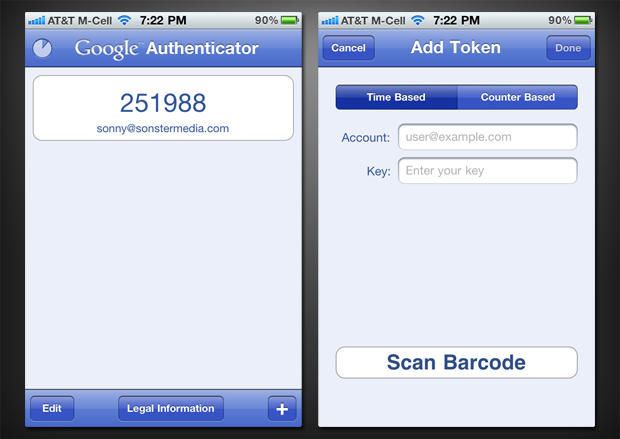
\includegraphics[scale=0.45]{GoogleAuthenticator_2.jpg}}
	    \caption{Google Authenticator}
	  \end{figure}  
  \end{itemize}
  \newpage
  OATH (Initiative for Open Authentication) Toolkit
  \begin{itemize}
    \item OATH Toolkit fournit une suite de composant pour la construction de systèmes d'authentification par mots de passe jetable. 
	  Les composant comprennent une librairie de programmation en C, un outil en lignes de commandes pour la génération et la validation d'OTP, et un PAM.
  \end{itemize}
  
  LinOTP
  \begin{itemize}
    \item LinOTP est une solution basée Linux pour gérer des systèmes d'authentifications à deux facteurs avec mots de passe jetables.
	  Il est implémenté comme un service web basé sur le framework python. C'est le seul serveur d'authentification open-source certifié par OATH.
	  \begin{figure}[h!]
	    \centerline{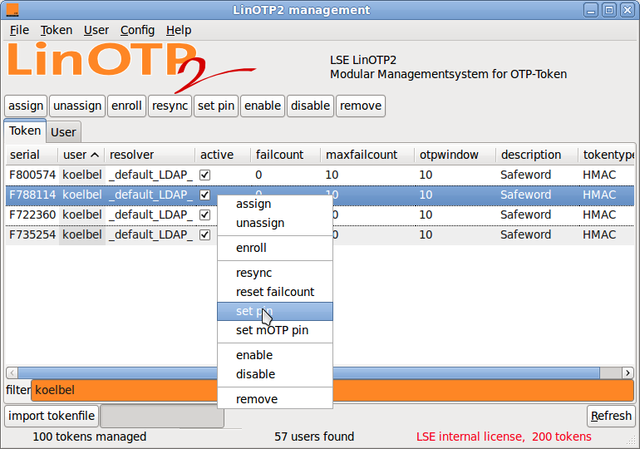
\includegraphics[scale=0.5]{linOTP.png}}
	  \end{figure}
  \end{itemize}  
  
  \subsection{Pérennité du système}
    Comme nous avons pu le voir, le système HOTP ne possède pas de faille de sécurité référencée. De plus, le système n'est pas affecté par les faiblesses des fonctions de 
    hachage, notamment au niveau des collisions. Ainsi, il est fortement envisageable que la fonction HMAC\_SHA\_1 puisse être utilisée pour générer des OTP pour une durée
    encore importante sans compromettre sa sécurité.
    
    De plus, si la fonction HMAC\_SHA\_1 se trouve dépréciée dans le futur, il suffirait de la remplacer par une nouvelle version reposant sur une fonction de hachage plus 
    forte telle que keccak ou whirlpool. Ce qui ne nécessiterait que peu de mises à jour.
    
    On peut donc considérer ce système de calcul d'OTP comme pérenne.
    
\end{document}
